


\begin{figure*}
    \begin{subfigure}[b]{0.49\textwidth}
    \centering
    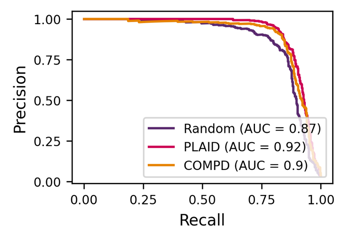
\includegraphics[width=\textwidth]{figures/PR-8-8-0.1-1.png}
    \caption{1\% hits}
    %\label{fig:plaid-control-layout-bowl}
  \end{subfigure}
  \hfill
  \begin{subfigure}[b]{0.49\textwidth}
    \centering
    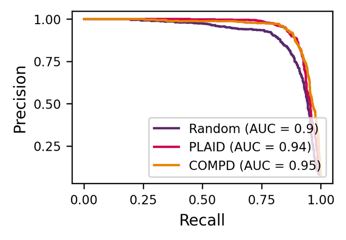
\includegraphics[width=\textwidth]{figures/PR-8-8-0.1-5.png}
    \caption{5\% hits}
    %\label{fig:plaid-control-layout-bowl}
  \end{subfigure}

  
  \begin{subfigure}[b]{0.49\textwidth}
    \centering
    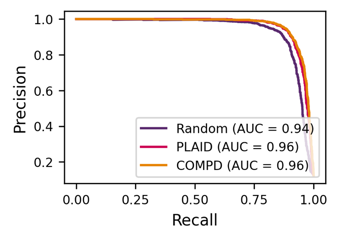
\includegraphics[width=\textwidth]{figures/PR-8-8-0.1-10.png}
    \caption{10\% hits}
    %\label{fig:plaid-control-layout-bowl}
  \end{subfigure}
  \hfill
  \begin{subfigure}[b]{0.49\textwidth}
    \centering
    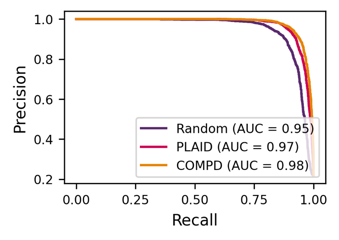
\includegraphics[width=\textwidth]{figures/PR-8-8-0.1-20.png}
    \caption{20\% hits}
    %\label{fig:plaid-control-layout-bowl}
  \end{subfigure}

  \begin{subfigure}[b]{0.49\textwidth}
    \centering
    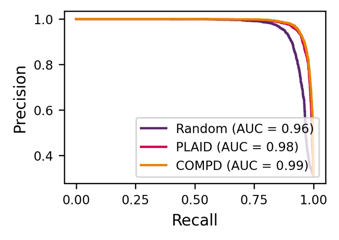
\includegraphics[width=\textwidth]{figures/PR-8-8-0.1-30.png}
    \caption{30\% hits}
    %\label{fig:plaid-control-layout-bowl}
  \end{subfigure}
  \hfill
  \begin{subfigure}[b]{0.49\textwidth}
    \centering
    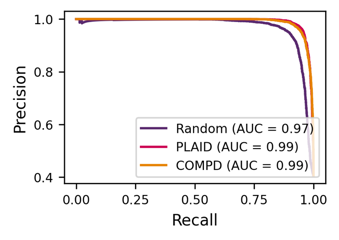
\includegraphics[width=\textwidth]{figures/PR-8-8-0.1-40.png}
    \caption{40\% hits}
    %\label{fig:plaid-control-layout-bowl}
  \end{subfigure}
  
  \caption{Comparison of PR curves for screening experiments with
    different hit rates, using layouts with 8 positive and 8
    negative controls in the presence of moderate bowl-shaped plate
    effects.}
    \label{fig:screening-pr-8-8}
\end{figure*}




%%% Local Variables: 
%%% mode: latex
%%% TeX-master: "../supplement.tex"
%%% End: 
